%%%%%%%%%%%%%%%%%%%%%%%%%%%%%%%%%%%%%%%%%
% Jacobs Landscape Poster
% LaTeX Template
%
% Original poster by:
% Computational Physics and Biophysics Group, Jacobs University
% https://teamwork.jacobs-university.de:8443/confluence/display/CoPandBiG/LaTeX+Poster
% 
% Also modified by:
% Nathaniel Johnston (nathaniel@njohnston.ca)
% Sarah Scheffler (sscheff@bu.edu, 4/26/17)
%
% This template has been downloaded from:
% http://www.LaTeXTemplates.com
%
% License:
% CC BY-NC-SA 3.0 (http://creativecommons.org/licenses/by-nc-sa/3.0/)
%
%%%%%%%%%%%%%%%%%%%%%%%%%%%%%%%%%%%%%%%%%

%----------------------------------------------------------------------------------------
%	PACKAGES AND OTHER DOCUMENT CONFIGURATIONS
%----------------------------------------------------------------------------------------

\documentclass[final]{beamer}

\usepackage[scale=1.24]{beamerposter} % Use the beamerposter package for laying out the poster

\usetheme{confposter} % Use the confposter theme supplied with this template

\setbeamercolor{block title}{fg=ngreen,bg=white} % Colors of the block titles
\setbeamercolor{block body}{fg=black,bg=white} % Colors of the body of blocks
\setbeamercolor{block alerted title}{fg=white,bg=dblue!70} % Colors of the highlighted block titles
\setbeamercolor{block alerted body}{fg=black,bg=dblue!10} % Colors of the body of highlighted blocks
% Many more colors are available for use in beamerthemeconfposter.sty

%-----------------------------------------------------------
% Define the column widths and overall poster size
% To set effective sepwid, onecolwid and twocolwid values, first choose how many columns you want and how much separation you want between columns
% In this template, the separation width chosen is 0.024 of the paper width and a 4-column layout
% onecolwid should therefore be (1-(# of columns+1)*sepwid)/# of columns e.g. (1-(4+1)*0.024)/4 = 0.22
% Set twocolwid to be (2*onecolwid)+sepwid = 0.464
% Set threecolwid to be (3*onecolwid)+2*sepwid = 0.708

\newlength{\sepwid}
\newlength{\onecolwid}
\newlength{\twocolwid}
\newlength{\threecolwid}
\setlength{\paperwidth}{48in} % A0 width: 46.8in
\setlength{\paperheight}{36in} % A0 height: 33.1in
\setlength{\sepwid}{0.024\paperwidth} % Separation width (white space) between columns
\setlength{\onecolwid}{0.22\paperwidth} % Width of one column
\setlength{\twocolwid}{0.464\paperwidth} % Width of two columns
\setlength{\threecolwid}{0.708\paperwidth} % Width of three columns
\setlength{\topmargin}{-0.5in} % Reduce the top margin size
%-----------------------------------------------------------

\usepackage{graphicx}  % Required for including images

\usepackage{booktabs} % Top and bottom rules for tables

%----------------------------------------------------------------------------------------
%	TITLE SECTION 
%----------------------------------------------------------------------------------------

\title{Measuring Security of Closed DNS Resolvers} % Poster title

\author{Sarah Scheffler, Sean Smith, Yossi Gilad, Sharon Goldberg} % Author(s) %TODO: ordering?

\institute{\{sscheff, swsmith, yossigi\}@bu.edu, goldbe@cs.bu.edu} % Institution(s)

%----------------------------------------------------------------------------------------

\begin{document}

\addtobeamertemplate{block end}{}{\vspace*{2ex}} % White space under blocks
\addtobeamertemplate{block alerted end}{}{\vspace*{2ex}} % White space under highlighted (alert) blocks

\setlength{\belowcaptionskip}{2ex} % White space under figures
\setlength\belowdisplayshortskip{2ex} % White space under equations

\begin{frame}[t] % The whole poster is enclosed in one beamer frame

\begin{columns}[t] % The whole poster consists of three major columns, the second of which is split into two columns twice - the [t] option aligns each column's content to the top

\begin{column}{\sepwid}\end{column} % Empty spacer column

\begin{column}{\onecolwid} % The first column


% PLANNING SECTION
% Goals
% Closed DNS resolvers and DNS checks made by email
% Measurement design
% Attacks from insecure DNS configurations

%		%				%
% Goals % Measurement	% attacks
% %	% % % design		% from
% closed%				% insecure
%resolv+%	 picture	% DNS
%		%				%

%----------------------------------------------------------------------------------------
%	OBJECTIVES
%----------------------------------------------------------------------------------------

%\begin{alertblock}{Objectives}

%Lorem ipsum dolor sit amet, consectetur, nunc tellus pulvinar tortor, commodo eleifend %risus arcu sed odio:
%\begin{itemize}
%\item Mollis dignissim, magna augue tincidunt dolor, interdum vestibulum urna
%\item Sed aliquet luctus lectus, eget aliquet leo ullamcorper consequat. Vivamus eros sem, %iaculis ut euismod non, sollicitudin vel orci.
%\item Nascetur ridiculus mus.  
%\item Euismod non erat. Nam ultricies pellentesque nunc, ultrices volutpat nisl ultrices a.
%\end{itemize}

%\end{alertblock}

%----------------------------------------------------------------------------------------
%	GOALS
%----------------------------------------------------------------------------------------

\begin{block}{Goals}

In response to the spread of cache poisoning attacks, many DNS resolvers have gone from being \emph{open} to \emph{closed} resolvers, meaning that they will only perform queries on behalf of hosts within a single organization or Internet Service Provider. As a result, measuring the security of the DNS infrastructure has been made more difficult. Closed resolvers will not respond to researcher queries to determine if they utilize security measures like port randomization or transaction id randomization. However, we can effectively turn a closed resolver into an open one by sending an email to a mail server (MTA) in the organization.  This causes the MTA to make a query on the external researchers' behalf, and we can log the security features of the DNS resolver using information gained by a nameserver and email server under our control. The goals of this experiment are
\vspace{-10px}
\begin{enumerate}
\item ~to measure the security of closed DNS resolvers using Email
\item ~to measure the relationship between MTAs and DNS resolvers that make queries on their behalf
\item ~to measure what DNS queries are made as a result of sending an email under several different spam-prevention measures
\end{enumerate}

\end{block}

%------------------------------------------------
%----------------------------------------------------------------------------------------
%	EMAIL SPAM PREVENTION CAUSES DNS LOOKUPS
%----------------------------------------------------------------------------------------

\begin{block}{Email Spam Prevention and DNS}

Mail servers cause several DNS queries to be made as anti-spam measures. This experiment measures the DNS queries caused by sending an email
\begin{enumerate}
\item ~by itself
\item ~under several different Sender Policy Framework (SPF) configurations
\item ~with DomainKeys Identified Mail (DKIM) and Domain Message Authentication Reporting \& Conformance (DMARC)
\end{enumerate}

%% Say something about SPF non-compliance?
We have found instances where SPF records are checked such a in a way that allows us to craft an infinite chain of DNS lookups. Such an attack could be the injection vector for a Kaminsky DNS cache poisoning attack. We will determine how many systems are vulnerable to such an attack.
\end{block}

%----------------------------------------------------------------------------------------

\end{column} % End of the first column

\begin{column}{\sepwid}\end{column} % Empty spacer column

\begin{column}{\twocolwid} % Begin a column which is two columns wide (column 2)

%----------------------------------------------------------------------------------------
%	Measurement design wide title
%----------------------------------------------------------------------------------------

\begin{block}{Measurement Design}
% This is just here for the title
\end{block} 

\begin{columns}[t,totalwidth=\twocolwid] % Split up the two columns wide column

\begin{column}{\onecolwid}\vspace{-.6in} % The first column within column 2 (column 2.1)

%----------------------------------------------------------------------------------------
%	MEASUREMENT FLOW
%----------------------------------------------------------------------------------------

\begin{block}{Measurement Flow}

\begin{figure}[experiment]
  \centering
  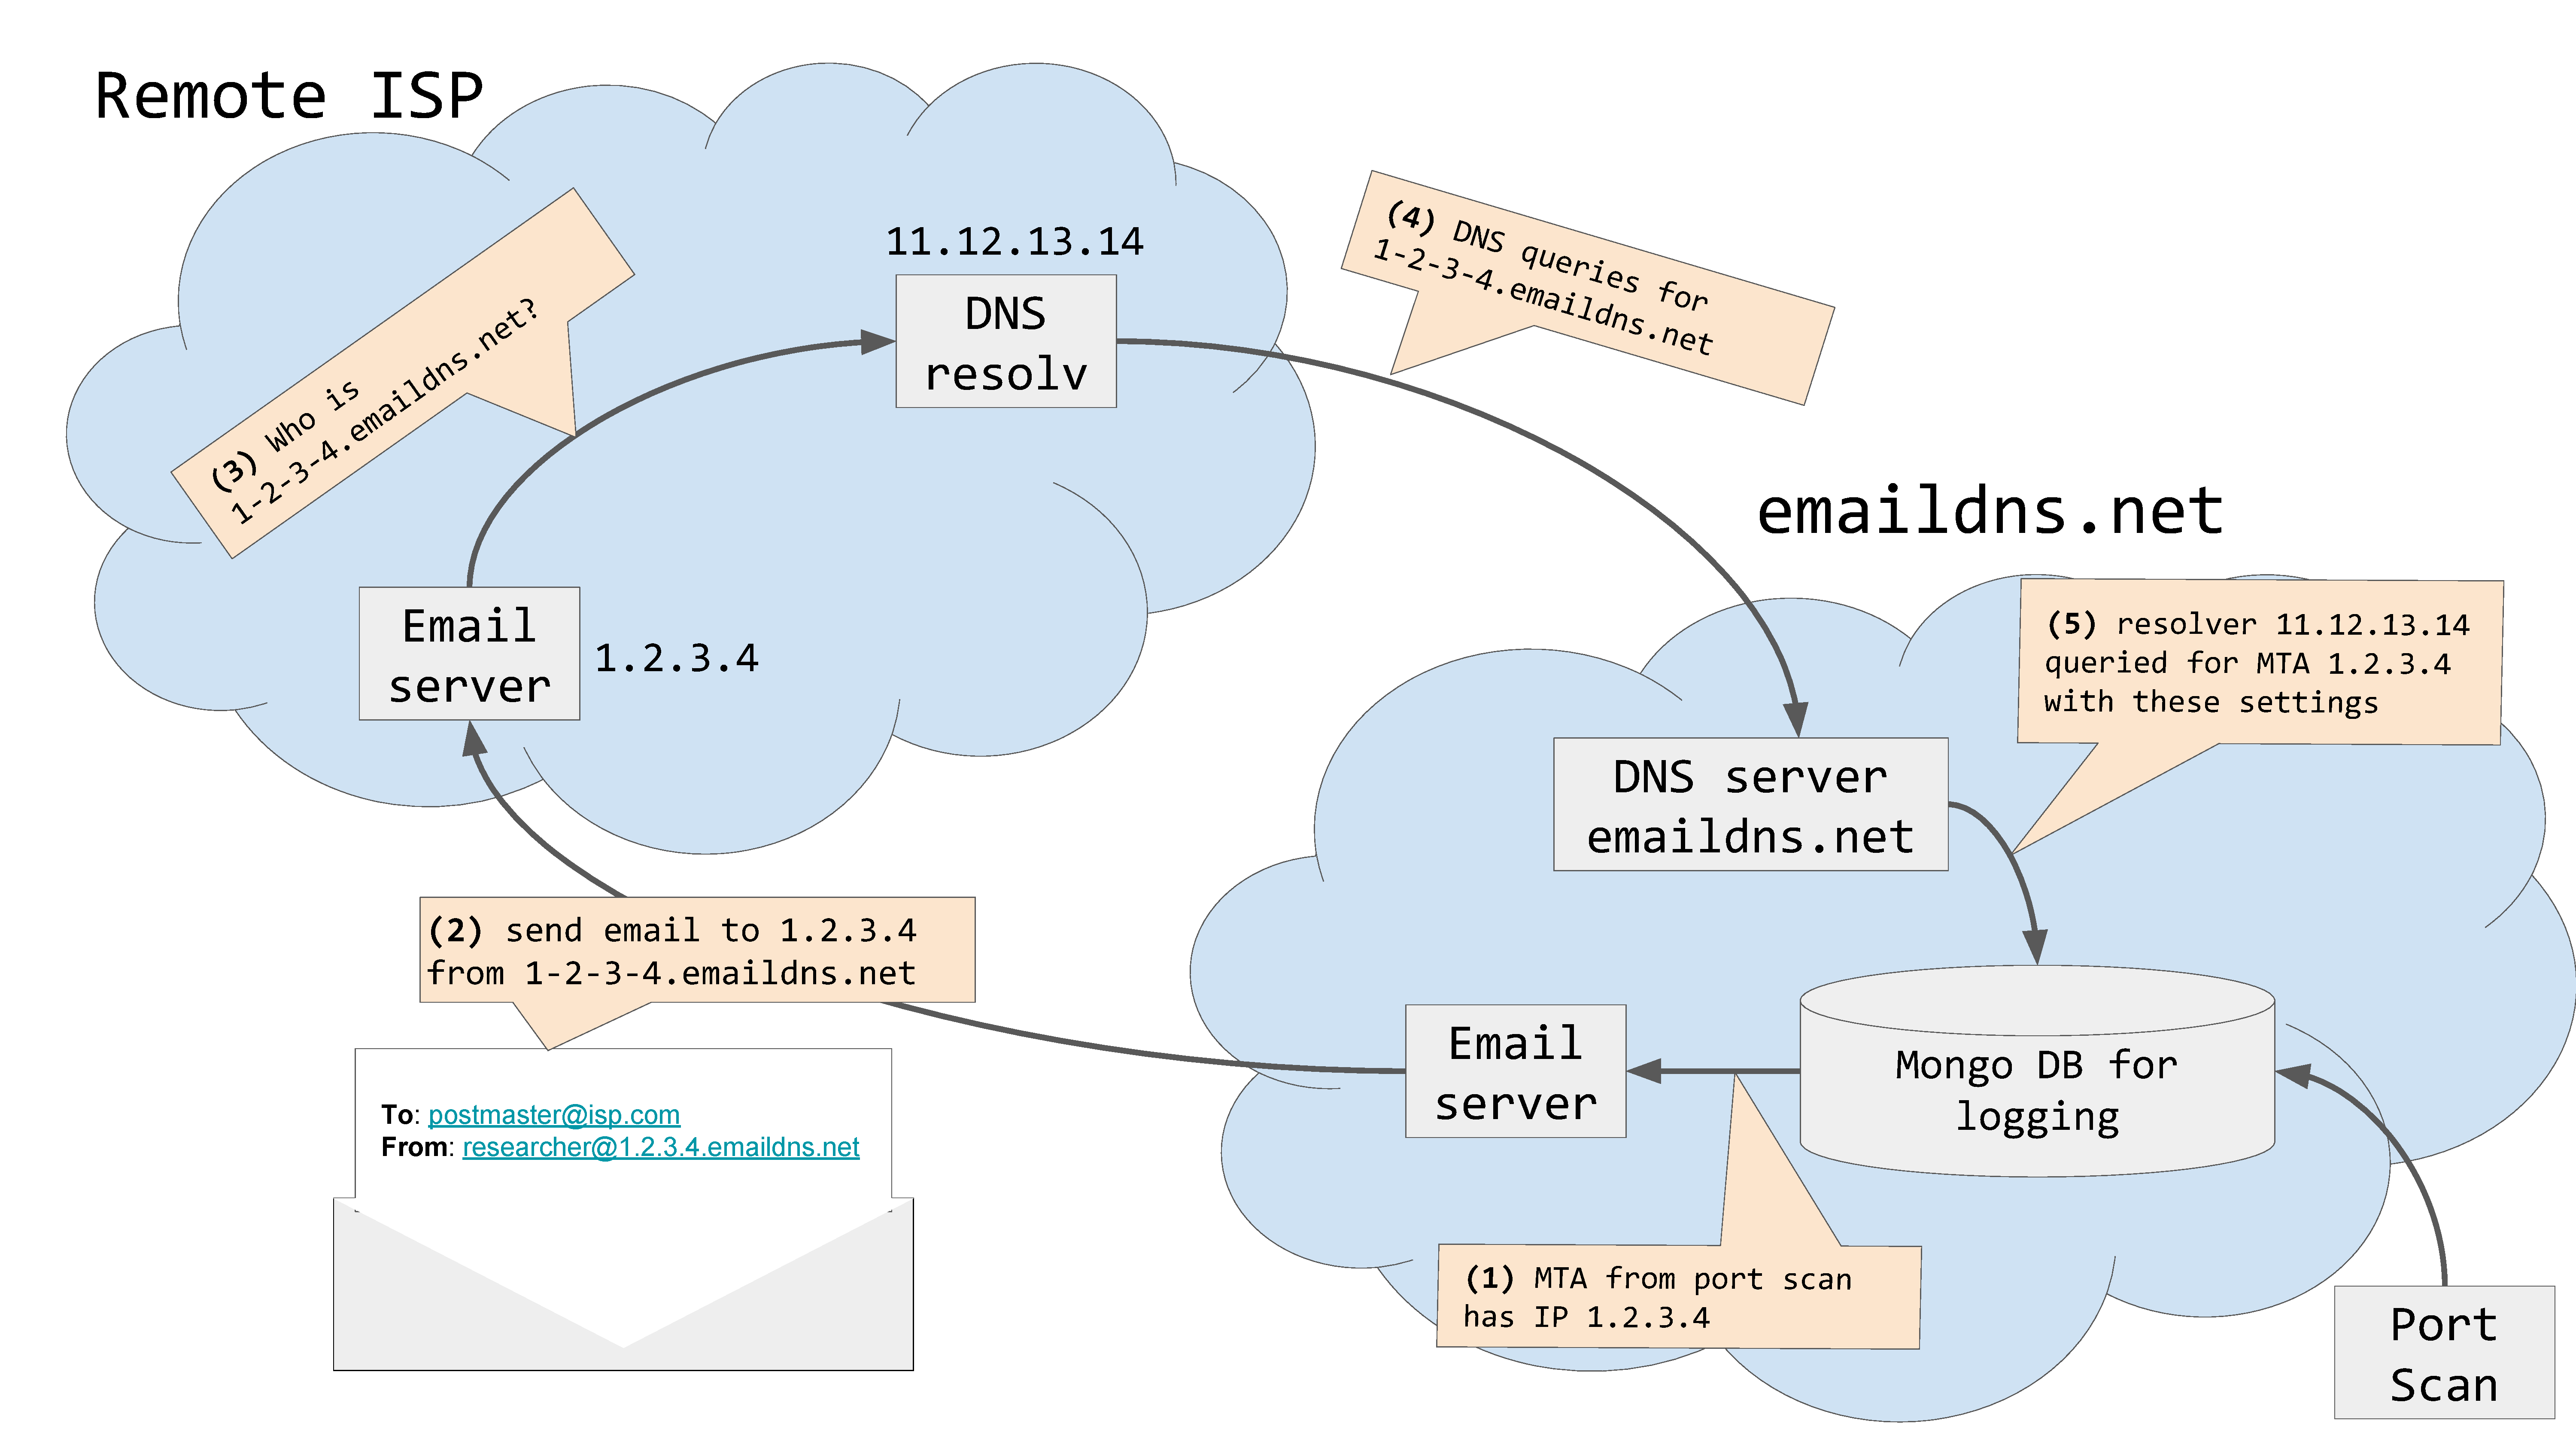
\includegraphics[width=\onecolwid]{experiment_flow}
  \caption{The experiment queries MTAs found in port scan, then measures what kinds of DNS queries were made from what servers in response.}
\end{figure}

\end{block}

%----------------------------------------------------------------------------------------
%	ANOTHER SECTION
%----------------------------------------------------------------------------------------

\begin{block}{DoS Amplification via SPF}

% We're doing an Internet wide scan with the purpose of exposing security vulnerabilities in the DNS architecture, stemming from the ability to turn a closed resolver into an open resolver. One such attack is an indirect DOS attack. 

Sender Policy framework (SPF) is an anti-spam email feature where the receiving MTA checks the DNS {\tt TXT} records of the domain sending the email. The {\tt TXT} record indicates which IP addresses are allowed to send email. 

One feature of SPF records allows you to specify {\tt include:anotherdomain.com} so that it recursively looks up another domain's SPF records. If this passes, the whole SPF record passes, but if it fails, it checks the next SPF record. The RFC states that the system must not lookup more than $10$ includes, but in practice, we've seen some mail servers check more than $10$ includes. Our attack is as follows:
\begin{itemize}
\item Send an email from {\tt us@ourdomain.com}
\item MTA looks up our SPF record in which we have $N$ include records {\tt include:anotherdomain.com}
\end{itemize}

We can change the length of $N$, have the SPF records include themselves, or have many nested includes to ourselves. Using these techniques we can create many DNS queries that come from the MTA and not directly from the attacker, bypassing some DoS defenses.
\end{block}


%----------------------------------------------------------------------------------------

\end{column} % End of column 2.1

\begin{column}{\onecolwid}\vspace{-.6in} % The second column within column 2 (column 2.2)

%----------------------------------------------------------------------------------------
%	OVERVIEW
%----------------------------------------------------------------------------------------

\begin{block}{Overview}

We send emails to MTAs, encoding information about the MTA in our sending address.  We then measure what queries were made to our nameserver, and from what IP addresses.  This enables us to determine which DNS resolver makes queries for which MTA, and by looking at repeated queries, we determine whether the resolver has security features like transaction id randomization and port randomization.

There are five phases to this experiment: %TODO: better intro here
\begin{enumerate}
\item ~Do an Internet-wide port scan on ports commonly used for SMTP (25, 465, 587, and 2525)
\item ~For each IP address in the scan, send an email to a recipient served by that MTA with a sending address that encodes the IP address of the MTA
\item ~The MTA will ask its DNS resolver to do some anti-spam checks on the given email address
\item ~The resolver asks our nameserver about the email address we sent from
\item ~Log all queries to our nameserver, they tell us:
\vspace{0.3cm}
\begin{itemize}
\item The IP address of the DNS resolver makes queries on behalf of this MTA
\vspace{0.2cm}
\item What anti-spam protection this MTA had implemented
\vspace{0.2cm}
\item Whether the DNS resolver had implemented security measures against cache poisoning, like port randomization or transaction id randomization
\end{itemize}
\end{enumerate}
Each of these steps must be done quickly to ensure that the public IP addresses of the MTAs and DNS resolvers do not change.

\end{block}

%----------------------------------------------------------------------------------------
%	GLOSSARY
%----------------------------------------------------------------------------------------

\begin{block}{Glossary}
\textbf{DNS} - Domain Name System

\textbf{MTA} - Mail Transfer Agent (Email server)

\textbf{SPF} - Sender Policy Framework (anti-spam measure implemented in some MTAs)
\end{block}


%----------------------------------------------------------------------------------------

\end{column} % End of column 2.2

\end{columns} % End of the split of column 2 - any content after this will now take up 2 columns width



%----------------------------------------------------------------------------------------

\begin{columns}[t,totalwidth=\twocolwid] % Split up the two columns wide column again

\begin{column}{\onecolwid} % The first column within column 2 (column 2.1)


%----------------------------------------------------------------------------------------

\end{column} % End of column 2.1

\begin{column}{\onecolwid} % The second column within column 2 (column 2.2)



%----------------------------------------------------------------------------------------

\end{column} % End of column 2.2

\end{columns} % End of the split of column 2

\end{column} % End of the second column

\begin{column}{\sepwid}\end{column} % Empty spacer column

\begin{column}{\onecolwid} % The third column

%----------------------------------------------------------------------------------------
%	DNS CACHE POISONING THROUGH EMAIL
%----------------------------------------------------------------------------------------

\begin{block}{DNS Cache Poisoning via Email}

\begin{figure}[cache_poisoning]
  \centering
  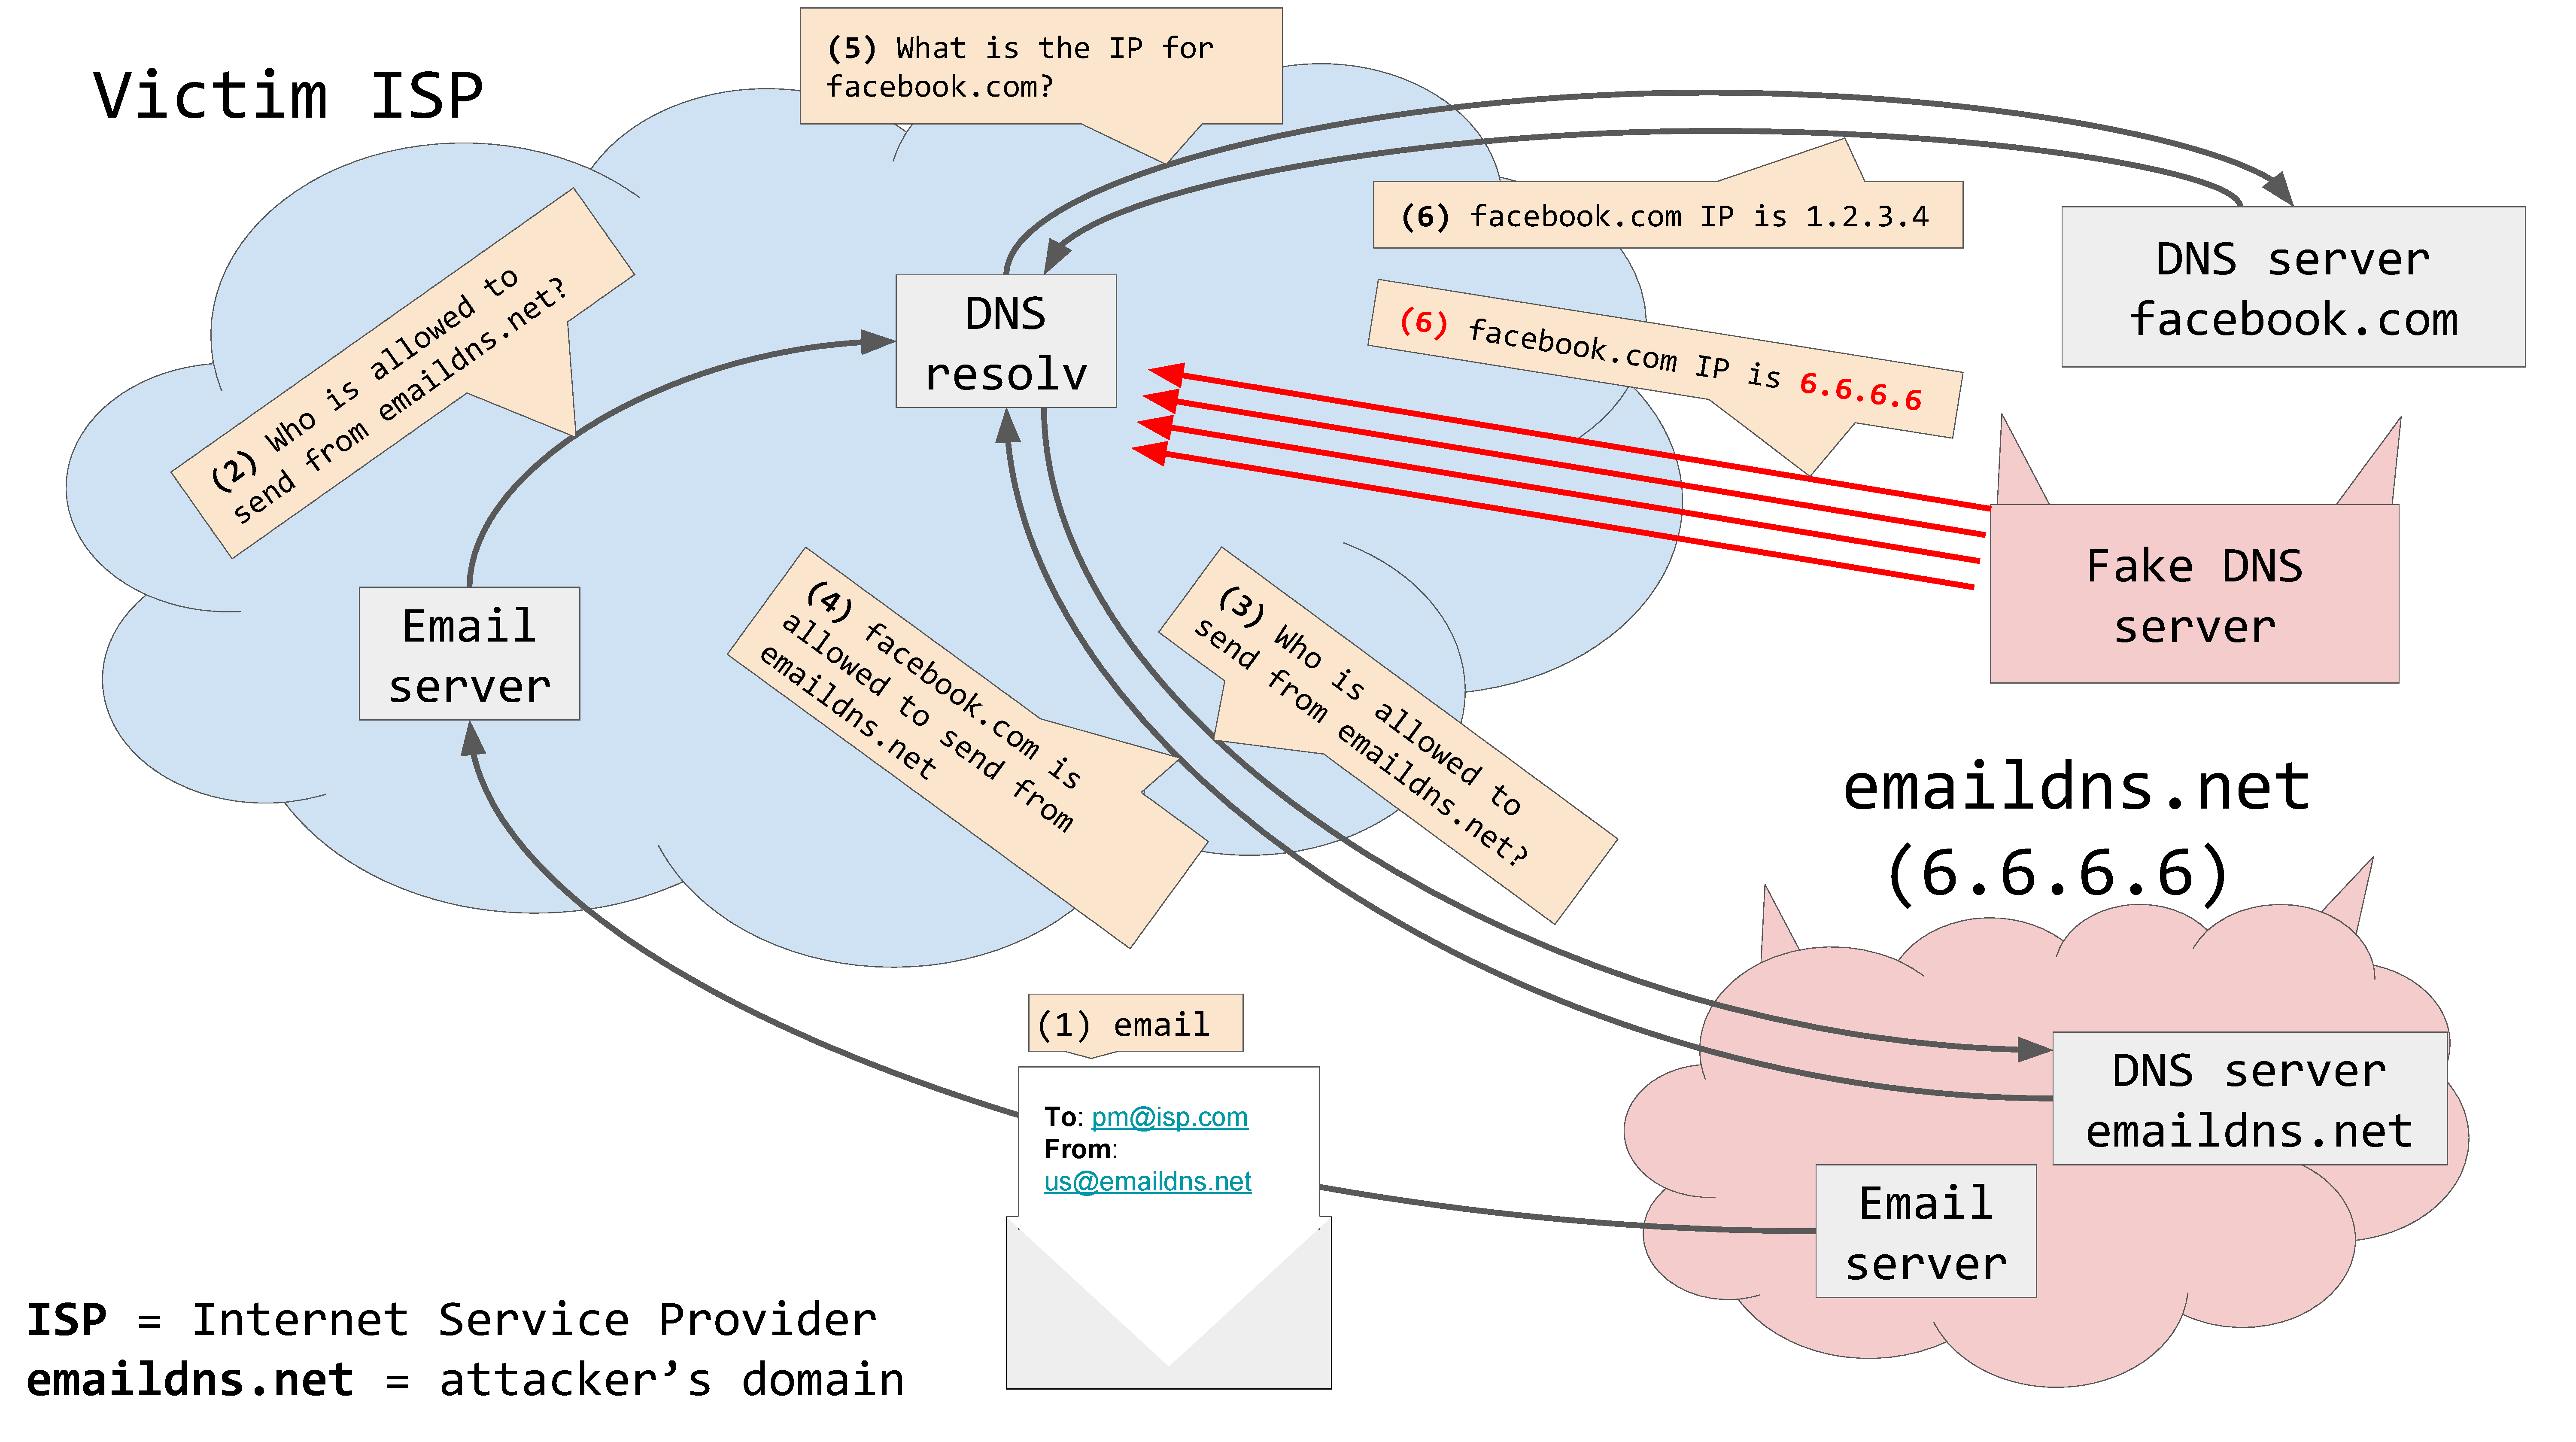
\includegraphics[width=\onecolwid]{Tim_Presentation}
  \caption{Executing a DNS cache poisoning attack on a closed resolver via Email}
\end{figure}

%TODO: cite kaminsky?
A Kaminsky attack "poisons" the cache of a DNS resolver by causing a query for an uncached subdomain and then sending a flood of packets to the resolver with fake responses claiming that that the IP address of the subdomain is a domain under the attacker's control.  Eventually, a benign response from the real domain will come as well, but it is discarded because the resolver already has the false answer in its cache.

In response to this attack, several ISPs closed their DNS resolvers to reduce the ability of the attacker to cause queries from their resolver.  Two other responses are \emph{port randomization} and \emph{transaction id randomization}, in which outgoing queries have their ports and transaction ids randomized, respectively.  The resolver only accepts a response if the transaction id and port match the transaction id and port from the query.  This forces the attacker to send a much larger amount of traffic in order to force one of their fraudulent packets to become the accepted answer. %TODO: actual numbers
One of our goals in this experiment is to determine the extent to which closed resolvers have implemented these randomization defenses.

\end{block}



%----------------------------------------------------------------------------------------
%	REFERENCES
%----------------------------------------------------------------------------------------

%\begin{block}{References}
%
%\nocite{*} % Insert publications even if they are not cited in the poster
%\small{\bibliographystyle{unsrt}
%\bibliography{sample}\vspace{0.75in}}
%
%\end{block}

%----------------------------------------------------------------------------------------
%	ACKNOWLEDGEMENTS
%----------------------------------------------------------------------------------------

\setbeamercolor{block title}{fg=red,bg=white} % Change the block title color

\begin{block}{Acknowledgements}

\small{\rmfamily{We thank Jared Mauch for his invaluable help in designing this experiment to be effective and repeatable, and for providing us infrastructure needs.  We also thank Timothy Edgar for discussions on the legal implications of the attacks proposed.}} 


\vspace*{\fill}
\begin{flushright}
\vspace{1cm}

\includegraphics[width=.1\linewidth]{bucompsci} \textsf{\large{~@BUCompSci}}
\end{flushright}

\end{block}


%----------------------------------------------------------------------------------------

\end{column} % End of the third column

\end{columns} % End of all the columns in the poster
s
\end{frame} % End of the enclosing frame

\end{document}
